\documentclass[border=0pt]{standalone}
\usepackage{lmodern}
\usepackage{tikz}
\usepackage{pgfplots}
\usepgfplotslibrary{groupplots}
\pgfplotsset{compat=1.17}
\definecolor{f07min}{HTML}{000000}
\definecolor{f07sg}{HTML}{0072B2}
\definecolor{f07arpls}{HTML}{D55E00}
\begin{document}
\begin{minipage}{181.86mm}
\centering
% figure: P08-F07; panel: f07-equal-context-m01-c-extra-trees; semantic-sha256: a80ccd58447783b6ff83336d15c300b5297f955760921573638eaca3cc08512e
{\bfseries\fontsize{10}{12}\selectfont P08-F07 / RQ-S05 | Extra Trees | M01 individual-spectrum predictions | Primary (P)\par}
\vspace{2mm}
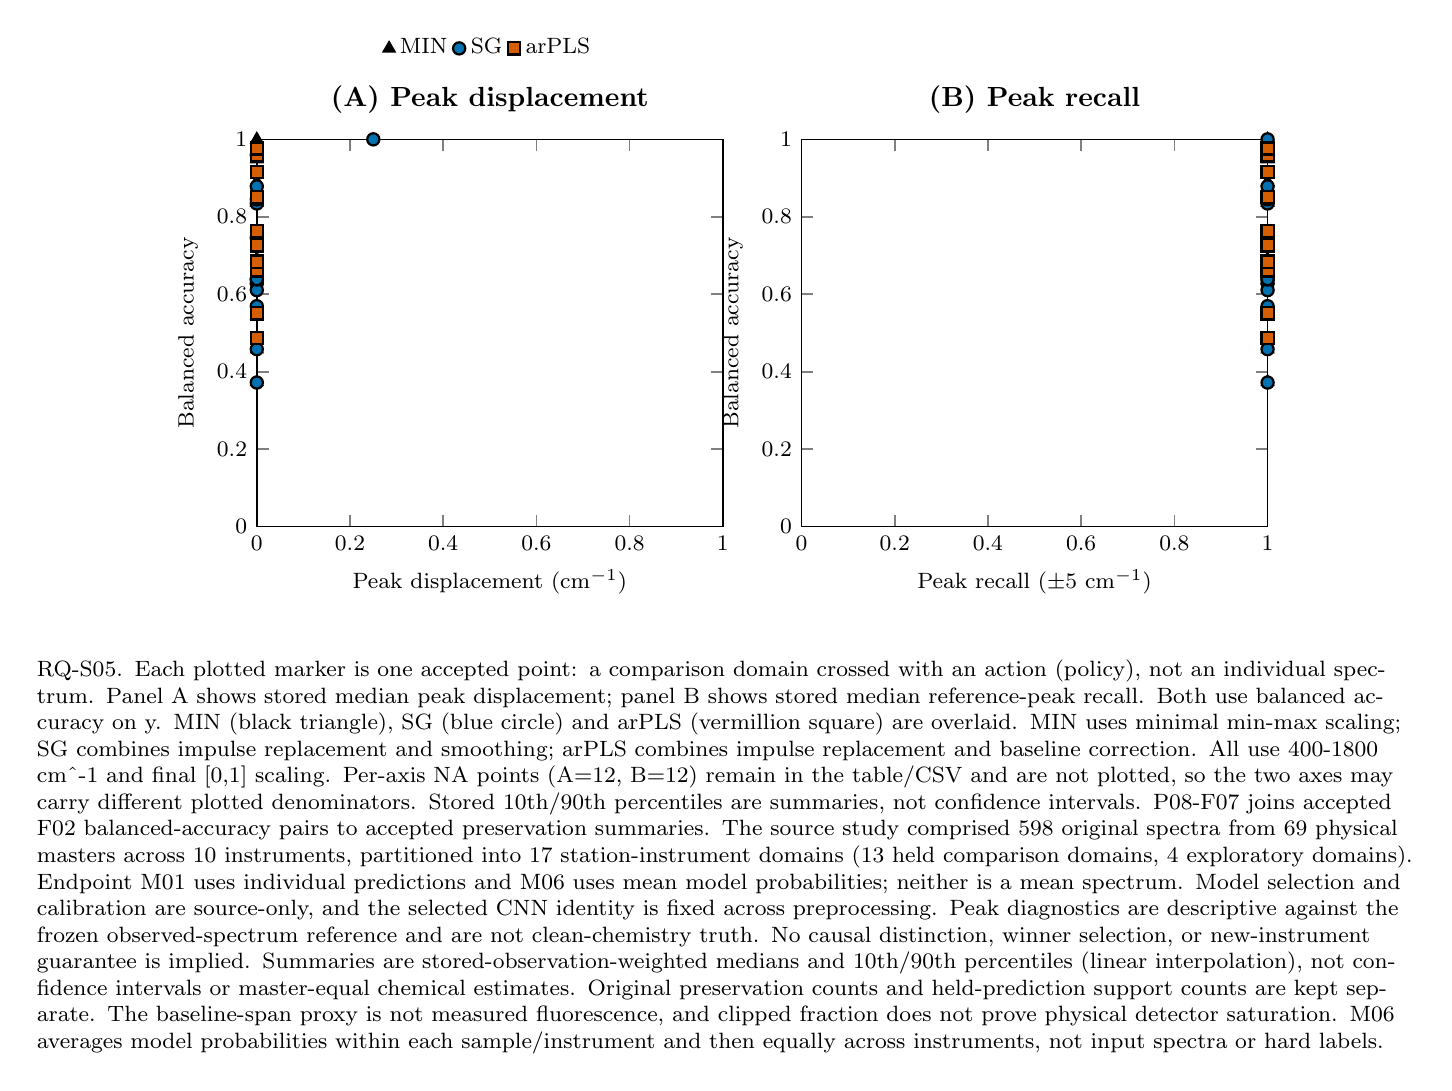
\begin{tikzpicture}
\begin{groupplot}[group style={group size=2 by 1, horizontal sep=10mm, vertical sep=0mm}, width=75mm, height=65mm, clip=false, axis line style={line width=0.6pt}, tick style={line width=0.6pt}, tick label style={font=\fontsize{8}{9.6}\selectfont, black}, label style={font=\fontsize{8}{9.6}\selectfont, black}, title style={font=\bfseries\fontsize{10}{12}\selectfont}, legend style={at={(0.5,1.18)}, anchor=south, draw=none, fill=none, legend columns=3, font=\fontsize{8}{9.6}\selectfont}, ymin=0, ymax=1, ytick={0,0.20000000000000001,0.40000000000000002,0.59999999999999998,0.80000000000000004,1}, yticklabels={0,0.2,0.4,0.6,0.8,1}]
\nextgroupplot[title={(A) Peak displacement}, xlabel={Peak displacement (cm$^{-1}$)}, ylabel={Balanced accuracy}, xmin=0, xmax=1, xtick={0,0.20000000000000001,0.40000000000000002,0.59999999999999998,0.80000000000000004,1}, xticklabels={0,0.2,0.4,0.6,0.8,1}]
\addlegendimage{only marks, mark=triangle*, mark size=2.2pt, mark options={fill=f07min, draw=black, line width=0.8pt}}
\addlegendentry{MIN}
\addlegendimage{only marks, mark=*, mark size=2.2pt, mark options={fill=f07sg, draw=black, line width=0.8pt}}
\addlegendentry{SG}
\addlegendimage{only marks, mark=square*, mark size=2.2pt, mark options={fill=f07arpls, draw=black, line width=0.8pt}}
\addlegendentry{arPLS}
\addplot+[only marks, mark=triangle*, mark size=2.2pt, mark options={fill=f07min, draw=black, line width=0.8pt}] coordinates {(0,0.68761784511784518) (0,0.63710317460317456) (0,0.69095238095238087) (0,0.84000000000000008) (0,0.94861111111111107) (0,0.37369708994708983) (0,0.83664682539682556) (0,1) (0,0.45833333333333337) (0,0.63646825396825391) (0,0.89035714285714307) (0,0.75974206349206341) (0,0.54490259740259739)};
\addplot+[only marks, mark=*, mark size=2.2pt, mark options={fill=f07sg, draw=black, line width=0.8pt}] coordinates {(0,0.62818722943722949) (0,0.61064814814814805) (0,0.63817460317460317) (0,0.83444444444444454) (0,0.95972222222222237) (0,0.37203042328042318) (0,0.84498015873015875) (0.25,1) (0,0.45833333333333337) (0,0.63924603174603167) (0,0.87857142857142867) (0,0.74529761904761904) (0,0.56922799422799431)};
\addplot+[only marks, mark=square*, mark size=2.2pt, mark options={fill=f07arpls, draw=black, line width=0.8pt}] coordinates {(0,0.66137265512265508) (0,0.55062169312169296) (0,0.72388888888888903) (0,0.85111111111111148) (0,0.97083333333333344) (0,0.68428240740740742) (0,0.85178571428571437) (0,0.95833333333333337) (0,0.48749999999999999) (0,0.72833333333333339) (0,0.97638888888888897) (0,0.76404761904761898) (0,0.91620250120250124)};
\nextgroupplot[title={(B) Peak recall}, xlabel={Peak recall ($\pm$5 cm$^{-1}$)}, ylabel={Balanced accuracy}, xmin=0, xmax=1, xtick={0,0.20000000000000001,0.40000000000000002,0.59999999999999998,0.80000000000000004,1}, xticklabels={0,0.2,0.4,0.6,0.8,1}]
\addplot+[only marks, mark=triangle*, mark size=2.2pt, mark options={fill=f07min, draw=black, line width=0.8pt}] coordinates {(1,0.68761784511784518) (1,0.63710317460317456) (1,0.69095238095238087) (1,0.84000000000000008) (1,0.94861111111111107) (1,0.37369708994708983) (1,0.83664682539682556) (1,1) (1,0.45833333333333337) (1,0.63646825396825391) (1,0.89035714285714307) (1,0.75974206349206341) (1,0.54490259740259739)};
\addplot+[only marks, mark=*, mark size=2.2pt, mark options={fill=f07sg, draw=black, line width=0.8pt}] coordinates {(1,0.62818722943722949) (1,0.61064814814814805) (1,0.63817460317460317) (1,0.83444444444444454) (1,0.95972222222222237) (1,0.37203042328042318) (1,0.84498015873015875) (1,1) (1,0.45833333333333337) (1,0.63924603174603167) (1,0.87857142857142867) (1,0.74529761904761904) (1,0.56922799422799431)};
\addplot+[only marks, mark=square*, mark size=2.2pt, mark options={fill=f07arpls, draw=black, line width=0.8pt}] coordinates {(1,0.66137265512265508) (1,0.55062169312169296) (1,0.72388888888888903) (1,0.85111111111111148) (1,0.97083333333333344) (1,0.68428240740740742) (1,0.85178571428571437) (1,0.95833333333333337) (1,0.48749999999999999) (1,0.72833333333333339) (1,0.97638888888888897) (1,0.76404761904761898) (1,0.91620250120250124)};
\end{groupplot}
\node[anchor=north, yshift=-6mm, text width=175mm, align=left, font=\fontsize{8}{9.6}\selectfont] at (current bounding box.south) {RQ-S05. Each plotted marker is one accepted point: a comparison domain crossed with an action (policy), not an individual spectrum. Panel A shows stored median peak displacement; panel B shows stored median reference-peak recall. Both use balanced accuracy on y. MIN (black triangle), SG (blue circle) and arPLS (vermillion square) are overlaid. MIN uses minimal min-max scaling; SG combines impulse replacement and smoothing; arPLS combines impulse replacement and baseline correction. All use 400-1800 cm\textasciicircum{}-1 and final [0,1] scaling. Per-axis NA points (A=12, B=12) remain in the table/CSV and are not plotted, so the two axes may carry different plotted denominators. Stored 10th/90th percentiles are summaries, not confidence intervals. P08-F07 joins accepted F02 balanced-accuracy pairs to accepted preservation summaries. The source study comprised 598 original spectra from 69 physical masters across 10 instruments, partitioned into 17 station-instrument domains (13 held comparison domains, 4 exploratory domains). Endpoint M01 uses individual predictions and M06 uses mean model probabilities; neither is a mean spectrum. Model selection and calibration are source-only, and the selected CNN identity is fixed across preprocessing. Peak diagnostics are descriptive against the frozen observed-spectrum reference and are not clean-chemistry truth. No causal distinction, winner selection, or new-instrument guarantee is implied. Summaries are stored-observation-weighted medians and 10th/90th percentiles (linear interpolation), not confidence intervals or master-equal chemical estimates. Original preservation counts and held-prediction support counts are kept separate. The baseline-span proxy is not measured fluorescence, and clipped fraction does not prove physical detector saturation. M06 averages model probabilities within each sample/instrument and then equally across instruments, not input spectra or hard labels.};
\end{tikzpicture}
\end{minipage}
\end{document}